\chapter{DASAR TEORI}
\par Bab ini menjelaskan dasar teori yang penulis gunakan sebagai landasan pengerjaan tugas akhir. Bab ini akan menjelaskan secara umum terkait istilah dan kakas bantu yang digunakan dalam pembuatan tugas akhir ini.

\section{Push Notification Terpusat}
\par Push Notification Terpusat merupakan aplikasi yang dibuat untuk memudahkan penyebaran informasi di lingkungan ITS sebagai pengganti media cetak \cite{application-thesis}. Aplikasi ini dapat mengirimkan push notification secara langsung atau terjadwal ke perangkat pengguna (Android dan iOS) \cite{application-thesis}. Push Notification Terpusat merupakan aplikasi yang akan dikembangkan dalam tugas akhir ini.

\section{iOS}
\par iOS adalah sistem operasi perangkat bergerak yang dikembangkan oleh Apple untuk perangkat iPhone, iPad, dan iPod \cite{ios-online}.
\par Pada tugas akhir ini, perangkat dengan sistem operasi iOS merupakan salah satu target penerima push notification yang dikirim oleh aplikasi push notification terpusat.

\section{Android}
\par Android adalah sistem operasi perangkat bergerak yang dikembangkan oleh Google untuk ponsel, pakaian, tablet, televisi, dan kendaraan \cite{android-online}.
\par Pada tugas akhir ini, perangkat dengan sistem operasi Android merupakan salah satu target penerima push notification yang dikirim oleh Push Notification Terpusat.

\section{Apple Push Notification Service (APNs)}
\par Apple Push Notification Service adalah layanan pengiriman notifikasi jarak jauh yang kuat, cepat dan sangat efisien, yang dapat digunakan oleh pengembang aplikasi untuk menyebarkan informasi ke perangkat iOS, watchOS, tvOS, dan macOS \cite{apns-online}.
\par Push notification yang menargetkan perangkat iOS akan dikirim ke layanan Apple Push Notification Service oleh Push Notification Terpusat.

\section{Firebase Cloud Messaging (FCM)}
\par Firebase Cloud Messaging adalah solusi pengiriman pesan lintas platform yang dapat diandalkan untuk mengirimkan pesan dan dapat digunakan tanpa biaya \cite{fcm-online}.
\par \textit{Push notification} yang menargetkan perangkat Android akan dikirim ke layanan Firebase Cloud Messaging oleh Push Notification Terpusat.

\section{Microsoft SQL Server}
\par Microsoft SQL Server adalah sistem basis data relasional yang bahasa pemrograman utamanya menggunakan MS-SQL dan Transact-SQL \cite{sqlserver-thesis}.
\par Pada tugas akhir ini, Microsoft SQL Server merupakan sistem basis data yang digunakan oleh Push Notification Terpusat.

\section{Message Queue}
\par \textit{Message queue} atau antrian pesan adalah metode komunikasi antar layanan secara asynchronous yang digunakan dalam arsitektur \textit{serverless} dan \textit{microservices}. Setiap pesan disimpan dalam antrian sampai pesan tersebut selesai diproses dan dihapus. Setiap pesan hanya diproses satu kali, oleh satu consumer \cite{message-queue-online}.
\par Pada tugas akhir ini, antrian pesan merupakan metode yang digunakan untuk menangani pengiriman \textit{push notification}. Perbandingan tanpa dan dengan antrian pesan dapat dilihat pada Tabel \ref{t:perbandingan-antrian-pesan}.
\begin{longtable}{|p{4.5cm}|p{4.5cm}|}
	\caption{Perbandingan Penggunaan Antrian Pesan} \label{t:perbandingan-antrian-pesan} \\ \hline
	\rowcolor{lightgray} Tanpa Antrian Pesan & Dengan Antrian Pesan \\ \hline
	Client dapat melihat langsung hasil \textit{request} & Client hanya mengetahui jika \textit{request} sudah tersimpan dan akan dijalankan \\ \hline
	Jika \textit{request} gagal, \textit{client} bertanggung jawab untuk mengulang operasi & Jika \textit{request} gagal, \textit{server} bertanggung jawab untuk mengulang operasi \\ \hline
	Spesifikasi sistem harus mencukupi penggunaan sumber daya & Penggunaan sumber daya dapat menyesuaikan spesifikasi sistem \\ \hline
\end{longtable}

\section{Apache Kafka}
\par Apache Kafka atau Kafka merupakan layanan terdistribusi untuk data streaming. Pada dasarnya, Kafka merupakan sistem \textit{publish/subscribe messaging}, dimana terdapat satu atau lebih sistem yang meng-\textit{generate} data untuk suatu topik tertentu secara \textit{real-time} di Kafka (disebut sebagai \textit{Producers}). Kemudian, topik tersebut dapat dibaca oleh satu atau lebih sistem yang membutuhkan data-data dari topik tersebut secara \textit{real-time} (disebut sebagai Consumers) \cite{kafka-online}.
\par Pada tugas akhir ini, Kafka akan digunakan sebagai pengganti antrian pesan Push Notification Terpusat. Tabel perbandingan antrian pesan Push Notification Terpusat dengan Apache Kafka dapat dilihat pada Tabel \ref{t:perbandingan_kafka}, dan arsitektur antrian pesan Push Notification Terpusat dan Apache Kafka pada Gambar \ref{img:arsitektur-mq_pnt} dan \ref{img:arsitektur-mq_kafka}.
\begin{longtable}{|p{2.5cm}|p{3.5cm}|p{3.5cm}|}
	\caption{Perbandingan Antrian Pesan Push Notification Terpusat dengan Apache Kafka} \label{t:perbandingan_kafka} \\ \hline
	\rowcolor{lightgray} & Push Notification Terpusat & Apache Kafka \\ \hline
	Penyimpanan pesan & \textit{Non Persistence}, disimpan dalam sistem (RAM) & \textit{Persistence}, disimpan dalam media penyimpanan perangkat (HDD atau SSD) \\ \hline
	Jumlah pesan maksimum & Dapat menangani 1.000 pesan tanpa gagal & Dapat menangani 1.000.000 pesan tanpa gagal \\ \hline
	Arsitektur antrian & Satu antrian untuk semua pesan & Antrian dibagi berdasarkan topik dan partisi \\ \hline
	Urutan pengambilan pesan & Terurut berdasarkan waktu ditambahkan & Jika di satu partisi, terurut berdasarkan waktu ditambahkan. Jika berbeda partisi, berdasarkan partisi manapun yang tidak kosong. \\ \hline
\end{longtable}
\begin{figure}[H]
\centering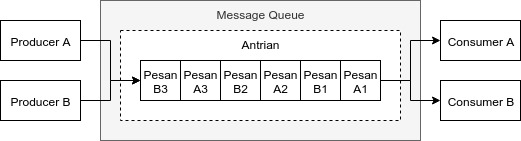
\includegraphics[width=0.75\textwidth]{bab2/img/arsitektur-mq_pnt.jpg}
\caption{Arsitektur Antrian Pesan Push Notification Terpusat}
\label{img:arsitektur-mq_pnt}
\end{figure}
\begin{figure}[H]
	\centering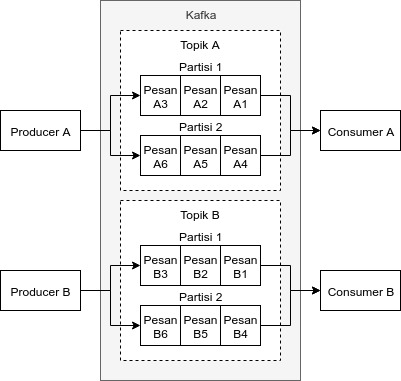
\includegraphics[width=0.75\textwidth]{bab2/img/arsitektur-mq_kafka.jpg}
	\caption{Arsitektur Antrian Pesan Apache Kafka}
	\label{img:arsitektur-mq_kafka}
\end{figure}

\section{Apache Zookeeper}
\par Apache Zookeeper atau Zookeeper adalah layanan tersentralisasi untuk mengatur konfigurasi, penamaan, sinkronisasi sistem terdistribusi, untuk sekelompok layanan \cite{zookeeper-online}.
\par Pada tugas akhir ini, Zookeeper merupakan layanan yang dibutuhkan oleh Kafka untuk beroperasi. Kafka menggunakan Zookeeper untuk mengatur koordinasi \textit{producer} dan \textit{consumer} dengan antrian pesan.

\section{Java}
\par Java adalah bahasa pemrograman yang umum, konkuren, berbasis kelas, dan berbasis objek \cite{java-online}.
\par Pada tugas akhir ini, Java merupakan bahasa pemrograman yang digunakan untuk implementasi Push Notification Terpusat. Alasan pemilihan Java adalah sebagai berikut:
\begin{enumerate}
	\item Mudah untuk dikembangkan
	\item Java didukung penuh oleh pengembang Kafka. Untuk bahasa lain, didukung oleh individu atau tim yang tidak resmi.
	\item Dokumentasi resmi Kafka menggunakan bahasa pemrograman Java.
\end{enumerate}

\section{Spring}
\par Spring adalah sebuah \textit{platform} yang menyediakan dukungan infrastruktur lengkap untuk mengembangkan aplikasi Java \cite{spring-online}. Spring merupakan kerangka kerja yang digunakan untuk mengembangkan Push Notification Terpusat.
\begin{enumerate}
	\item Dukungan pustaka untuk SQL Server dan Kafka.
\end{enumerate}

\section{Actuator}
\par Actuator berisi sekumpulan fitur tambahan untuk pemantauan dan pengaturan aplikasi yang sudah ditahap \textit{production}. Aplikasi bisa dipantau dan diatur dengan menggunakan \textit{endpoint} HTTP atau JMX \cite{actuator-online}.
\par Pada tugas akhir ini, Actuator merupakan pustaka yang digunakan dalam implementasi pemantauan Push Notification Terpusat.

\section{JSON}
\par JSON adalah format pertukaran data yang ringan, berbasis teks, dan independen \cite{json-online}.
\par Pada tugas akhir ini, JSON merupakan format pertukaran data yang digunakan oleh Kafka untuk menyimpan data, dan pustaka Actuator untuk menampilkan \textit{response}.

\section{Docker}
\par Docker adalah \textit{platform} terbuka untuk membangun, mengirim, dan menjalankan aplikasi. Docker memungkinkan pengembang untuk memisahkan kebutuhan infrastruktur dari aplikasi, sehingga proses pengembangan aplikasi bisa lebih cepat \cite{docker-online}.
\par Pada tugas akhir ini, Docker akan digunakan untuk menjalankan Push Notification Terpusat, Kafka, dan Zookeeper. Perbandingan penggunaan Docker dapat dilihat pada Tabel \ref{t:perbandingan_docker}, dan arsitektur Docker pada Gambar \ref{img:arsitektur-docker}.
\begin{longtable}{|p{2.5cm}|p{3.5cm}|p{3.5cm}|}
	\caption{Perbandingan Penggunaan Docker} \label{t:perbandingan_docker} \\ \hline
	\rowcolor{lightgray} & Tanpa Docker & Dengan Docker \\ \hline
	Proses \textit{deployment} & Membutuhkan konfigurasi khusus untuk setiap sistem operasi & Dapat langsung dijalankan di sistem operasi manapun \\ \hline
	Pembatasan sumber daya & Tidak terbatas & Penggunaan CPU dan Memori bisa dibatasi \\ \hline
	Sekuritas & Bergantung pada konfigurasi sistem operasi & \textit{Isolated}, bergantung pada konfigurasi Docker \\ \hline
\end{longtable}
\begin{figure}[H]
\centering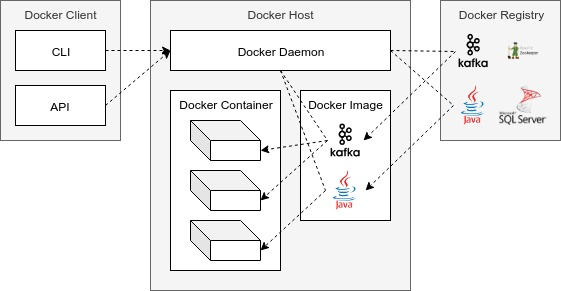
\includegraphics[width=0.75\textwidth]{bab2/img/arsitektur-docker.jpg}
\caption{Arsitektur Docker}
\label{img:arsitektur-docker}
\end{figure}

\section{Docker Compose}
\par Docker Compose adalah alat untuk mendefinisikan dan menjalankan beberapa \textit{container} aplikasi menggunakan Docker. Dengan Docker Compose, pengembang bisa menggunakan file berbasis YAML untuk mengatur konfigurasi layanan aplikasi, dan menggunakannya untuk membuat dan menjalankan layanan aplikasi \cite{docker-compose-online}.
\par Pada tugas akhir ini, Docker Compose akan digunakan untuk mendefinisikan konfigurasi yang digunakan untuk menjalankan Push Notification Terpusat, Kafka, dan Zookeeper. Perbandingan penggunaan Docker Compose dapat dilihat pada Tabel \ref{t:perbandingan_docker_compose}.
\begin{longtable}{|p{2cm}|p{3.5cm}|p{3.5cm}|}
	\caption{Perbandingan Penggunaan Docker Compose} \label{t:perbandingan_docker_compose} \\ \hline
	\rowcolor{lightgray} & Tanpa Compose & Dengan Compose \\ \hline
\end{longtable}

\section{YAML}
\par YAML adalah bahasa untuk serialisasi data yang dirancang agar mudah dipahami oleh manusia dan bisa berjalan dengan bahasa pemrograman modern \cite{yaml-online}.
\par Pada tugas akhir ini, YAML merupakan bahasa yang digunakan oleh Spring dan Docker Compose untuk mendefinisikan konfigurasi yang digunakan untuk menjalankan aplikasi.
